% Provenance (never printed): see sources/outline_sources.md (Year 1: crystal
% chemistry of minerals, silicates, solid solutions, mineral formulas, the main
% rock-forming minerals). Olivine curves in figdata/bachelor-1/solid_solution.py;
% the olivine analysis of the problem is invented (Fo about 82); exercise and
% problem values in the Book 3 scratch calculator calc/ch07.py.
\chapter{Minerales formadores de rocas}\label{ch:b1:rock-forming-minerals}

Una encimera de granito muestra tres o cuatro tipos de grano: cuarzo gris vítreo, \omterm{def:b1:rock-forming-minerals:groups}{feldespato} rosa o
blanco, láminas de \omterm{def:b1:rock-forming-minerals:groups}{mica} negra. La arena de playa es casi toda cuarzo. Los pequeños cristales verdes
dispersos en un basalto son \omterm{def:b1:rock-forming-minerals:groups}{olivino}, y el mismo \omterm{def:b1:rock-forming-minerals:mineral}{mineral}, con una composición algo distinta, forma la
mayor parte del manto superior. Unos pocos \omterm{def:b1:rock-forming-minerals:mineral}{minerales} construyen casi todas las rocas, y casi todos son
silicatos: oxígeno y silicio, los dos elementos más abundantes de la corteza, unidos en tetraedros que se
enlazan de unas pocas maneras sencillas. Este capítulo explica cómo el enlace fija la fórmula y el hábito
de un silicato, cómo un elemento reemplaza a otro en un cristal de modo que un \omterm{def:b1:rock-forming-minerals:mineral}{mineral} es una franja de
composiciones y no una sola, cómo un análisis químico se convierte en una fórmula, y cuáles son los
principales \omterm{def:b1:rock-forming-minerals:mineral}{minerales} formadores de rocas. Termina con un \omterm{def:b1:rock-forming-minerals:groups}{olivino} de un basalto, analizado, recalculado y pesado.

\begin{recall}
Un cristal es un sólido cuyos átomos se repiten en una red; la celda unidad es la caja más pequeña que
se repite, y el número de coordinación de un ion cuenta sus vecinos más próximos de carga opuesta
(química, primer año universitario). Los radios iónicos dependen de la carga y de la coordinación. Un
\omterm{def:b1:rock-forming-minerals:mineral}{mineral} se identifica en la mano por su hábito, su exfoliación, su dureza y su brillo (libro 2, año 11).
La cantidad de sustancia se cuenta en moles, y una masa molar es la masa de un mol (química).
\end{recall}

\section{Qué es un mineral}

\begin{definition}[Mineral]\label{def:b1:rock-forming-minerals:mineral}
Un \emph{mineral}\index{mineral} es un sólido de origen natural con una estructura cristalina definida y
una composición química que es fija o varía dentro de límites definidos. Casi todos los minerales son
inorgánicos.
\end{definition}

Una roca, en cambio, es un agregado de granos de uno o varios \omterm{def:b1:rock-forming-minerals:mineral}{minerales} (o de vidrio): el granito es
cuarzo, \omterm{def:b1:rock-forming-minerals:groups}{feldespatos} y \omterm{def:b1:rock-forming-minerals:groups}{mica}; la caliza es sobre todo calcita. Las dos mitades de la definición son
independientes. El vidrio de una ventana tiene la composición de un silicato pero no estructura
cristalina: no es un \omterm{def:b1:rock-forming-minerals:mineral}{mineral}, como tampoco lo es el vidrio de una lava enfriada bruscamente. Al revés,
la misma composición puede cristalizar en varias estructuras, y cada estructura es un \omterm{def:b1:rock-forming-minerals:mineral}{mineral} distinto.

\begin{definition}[Polimorfo]\label{def:b1:rock-forming-minerals:polymorph}
Dos \omterm{def:b1:rock-forming-minerals:mineral}{minerales} son \emph{polimorfos}\index{polimorfo} entre sí cuando tienen la misma composición química
y distinta estructura cristalina.
\end{definition}

El carbono cristaliza como grafito, un apilamiento de láminas de hexágonos con una densidad de
\qty{2.16}{g.cm^{-3}}, y como diamante, una red en la que cada átomo tiene cuatro vecinos, con una
densidad de \qty{3.51}{g.cm^{-3}}. El carbonato cálcico es calcita (\qty{2.71}{g.cm^{-3}}) o aragonito
(\qty{2.93}{g.cm^{-3}}); la sílice es cuarzo (\qty{2.65}{g.cm^{-3}}) o coesita
(\qty{2.93}{g.cm^{-3}}); \ce{Al2SiO5} es cianita (\qty{3.61}{g.cm^{-3}}), andalucita
(\qty{3.15}{g.cm^{-3}}) o sillimanita (\qty{3.24}{g.cm^{-3}}).
% ledger: webmineral:polymorphs, hom:calcite, hom:quartz
En cada pareja, el \omterm{def:b1:rock-forming-minerals:polymorph}{polimorfo} más denso es el que se forma a mayor presión: a una temperatura dada, subir la
presión favorece el estado de menor volumen (química, el desplazamiento de un equilibrio). El diamante en
una kimberlita y la coesita en una roca alcanzada por un meteorito registran, por tanto, presiones que solo se
encuentran en lo profundo del manto o en un impacto. Los tres \omterm{def:b1:rock-forming-minerals:polymorph}{polimorfos} del \ce{Al2SiO5}, cuyos campos de
estabilidad reparten entre ellos el plano presión--temperatura, sirven para leer las condiciones del
metamorfismo (segundo año universitario).

\section{El tetraedro de silicio y sus enlaces}

En casi todos los silicatos comunes, cada átomo de silicio está en el centro de cuatro átomos de oxígeno
colocados en los vértices de un tetraedro regular: la unidad \ce{SiO4} recordada de la química. El ion
silicio es pequeño (\qty{0.26}{\angstrom} en coordinación cuádruple) y el ion óxido es grande, así que
caben cuatro oxígenos alrededor del silicio y no más; el enlace silicio--oxígeno es fuerte y en parte
covalente. Una unidad aislada lleva una carga $4 - 4\times2 = -4$.
% ledger: shannon:radii
Los tetraedros pueden ir aislados, con su carga equilibrada por cationes metálicos entre ellos, o compartir
vértices: un oxígeno común a dos tetraedros es un \emph{oxígeno puente}. Dos tetraedros nunca comparten una
arista ni una cara, lo que acercaría demasiado dos silicios. Los silicatos se clasifican según el número de
vértices que comparte cada tetraedro (\cref{def:b1:rock-forming-minerals:silicate-classes}).

\begin{omfigure}
\tikzset{
  tup/.pic={\filldraw[fill=omLithLime, draw=black, line join=round] (0,0) -- (1,0) -- (0.5,0.866) -- cycle;
            \fill[omThm] (0.5,0.2887) circle (0.11);},
  tdn/.pic={\filldraw[fill=omLithLime, draw=black, line join=round] (0,0) -- (1,0) -- (0.5,-0.866) -- cycle;
            \fill[omThm] (0.5,-0.2887) circle (0.11);},
  linkpanel/.style={x=0.45cm, y=0.45cm, baseline=(current bounding box.south)}}
\setlength{\tabcolsep}{4pt}
\begin{tabular}{cccc}
% (a) the tetrahedron in perspective
\begin{tikzpicture}[linkpanel]
  \useasboundingbox (-1.2,-1.0) rectangle (6.0,4.4);
  \coordinate (T) at (2.2,3.7); \coordinate (L) at (0.3,0.5); \coordinate (R) at (4.1,0.1);
  \coordinate (B) at (3.3,2.1); \coordinate (C) at (2.475,1.6);
  \draw[densely dashed, gray] (L) -- (B) -- (R) (B) -- (T);
  \shade[ball color=omLithShale] (B) circle (0.42);
  \draw[gray] (C) -- (T) (C) -- (L) (C) -- (R) (C) -- (B);
  \shade[ball color=omThm!70] (C) circle (0.24);
  \draw[thick, line join=round] (T) -- (L) -- (R) -- cycle;
  \foreach \p in {T,L,R} \shade[ball color=omLithShale] (\p) circle (0.42);
  \node[right] at (4.5,0.1) {\scriptsize O};
  \node[right] at (2.6,3.8) {\scriptsize O};
  \draw[omThm] (C) -- (4.6,2.2) node[right] {\scriptsize Si};
\end{tikzpicture} &
% (b) nesosilicate: isolated tetrahedra
\begin{tikzpicture}[linkpanel]
  \useasboundingbox (-1.2,-1.0) rectangle (6.0,4.4);
  \pic at (0,0.3) {tup}; \pic at (2.4,0.3) {tup}; \pic at (4.0,1.9) {tdn};
  \pic at (1.2,2.4) {tdn}; \pic at (3.0,2.8) {tup};
\end{tikzpicture} &
% (c) sorosilicate: pairs
\begin{tikzpicture}[linkpanel]
  \useasboundingbox (-1.2,-1.0) rectangle (6.0,4.4);
  \pic at (0,0.9) {tup}; \pic at (1,0.9) {tdn};
  \pic at (2.6,2.6) {tup}; \pic at (3.6,2.6) {tdn};
\end{tikzpicture} &
% (d) cyclosilicate: a ring of six
\begin{tikzpicture}[linkpanel]
  \useasboundingbox (-1.2,-1.0) rectangle (6.0,4.4);
  \begin{scope}[shift={(2.4,1.7)}]
  \foreach \t in {0,60,...,300} {
    \filldraw[fill=omLithLime, draw=black, line join=round] (\t-30:1) -- (\t+30:1) -- (\t:1.732) -- cycle;
    \fill[omThm] (\t:1.155) circle (0.11);}
  \end{scope}
\end{tikzpicture} \\
  {\small (a) el tetraedro \ce{SiO4}} & {\small (b) \omterm{def:b1:rock-forming-minerals:silicate-classes}{nesosilicato}} & {\small (c) \omterm{def:b1:rock-forming-minerals:silicate-classes}{sorosilicato}} & {\small (d) \omterm{def:b1:rock-forming-minerals:silicate-classes}{ciclosilicato}} \\
 & {\scriptsize $s = 0$, \ce{SiO4}} & {\scriptsize $s = 1$, \ce{Si2O7}} & {\scriptsize $s = 2$, \ce{Si6O18}} \\[6pt]
% (e) single chain
\begin{tikzpicture}[linkpanel]
  \useasboundingbox (-0.6,-1.2) rectangle (7.6,4.6);
  \begin{scope}[shift={(0,1.5)}]
  \foreach \i in {0,...,3} \pic at (2*\i,0) {tup};
  \foreach \i in {0,...,2} \pic at (2*\i+1,0) {tdn};
  \end{scope}
\end{tikzpicture} &
% (f) double chain: two single chains joined through every other apex
\begin{tikzpicture}[linkpanel]
  \useasboundingbox (-0.6,-1.2) rectangle (7.6,4.6);
  \begin{scope}[shift={(0.5,0.4)}]
  \foreach \i in {0,...,3} {\pic at (2*\i,0) {tup}; \pic at (2*\i,1.732) {tdn};}
  \foreach \i in {0,...,2} {\pic at (2*\i+1,0) {tdn}; \pic at (2*\i+1,1.732) {tup};}
  \end{scope}
\end{tikzpicture} &
% (g) sheet
\begin{tikzpicture}[linkpanel]
  \useasboundingbox (-0.6,-1.2) rectangle (7.6,4.6);
  \foreach \j in {0,1,2} {
    \foreach \i in {0,1,2} {\pic at (2*\i+\j,1.732*\j) {tup};}
    \foreach \i in {0,1} {\pic at (2*\i+\j+1,1.732*\j) {tdn};}}
\end{tikzpicture} &
% (h) framework: a sheet whose apices point alternately up and down
\begin{tikzpicture}[linkpanel]
  \useasboundingbox (-0.6,-1.2) rectangle (7.6,4.6);
  \foreach \j in {0,1,2} {
    \foreach \i in {0,1,2} {\pic at (2*\i+\j,1.732*\j) {tup};}
    \foreach \i in {0,1} {\pic at (2*\i+\j+1,1.732*\j) {tdn};}}
  \foreach \j in {0,1,2} \foreach \i in {0,1} {
    \filldraw[fill=white, draw=omThm, thick] (2*\i+\j+1.5,1.732*\j-0.2887) circle (0.17);}
\end{tikzpicture} \\
{\small (e) cadena simple} & {\small (f) cadena doble} & {\small (g) lámina} & {\small (h) armazón} \\
{\scriptsize $s = 2$, \ce{SiO3}} & {\scriptsize $s = 2$ y $3$, \ce{Si4O11}} & {\scriptsize $s = 3$, \ce{Si2O5}} & {\scriptsize $s = 4$, \ce{SiO2}} \\
\end{tabular}
\medskip

{\small El tetraedro \ce{SiO4} (a) y las maneras en que los tetraedros se enlazan, vistas desde arriba:
cada triángulo es la base de un tetraedro, con tres oxígenos en sus vértices, y el cuarto encima del
punto, que marca el silicio. Los vértices que se tocan son oxígenos compartidos; $s$ es el número de
vértices que comparte cada tetraedro. En el armazón (h), los oxígenos de los vértices (círculos vacíos:
apuntan hacia abajo; puntos: hacia arriba) también se comparten, con las láminas inferior y superior.}
\end{omfigure}

\begin{definition}[Las clases de silicatos]\label{def:b1:rock-forming-minerals:silicate-classes}
Los silicatos se clasifican según cómo se enlazan sus tetraedros \ce{SiO4}. En un
\emph{nesosilicato}\index{nesosilicato} los tetraedros están aislados; en un
\emph{sorosilicato}\index{sorosilicato} se enlazan de dos en dos por un oxígeno compartido; en un
\emph{ciclosilicato}\index{ciclosilicato} forman anillos cerrados, cada uno con dos vértices compartidos;
en un \emph{inosilicato}\index{inosilicato} forman cadenas sin fin, simples (cada tetraedro comparte dos
vértices) o dobles (dos cadenas simples unidas lado a lado, con la mitad de los tetraedros compartiendo
tres vértices); en un \emph{filosilicato}\index{filosilicato} forman láminas sin fin, cada una con tres
vértices compartidos; en un \emph{tectosilicato}\index{tectosilicato} forman un armazón tridimensional,
con los cuatro vértices compartidos.
\end{definition}

\begin{proposition}[La razón silicio a oxígeno]\label{prop:b1:rock-forming-minerals:si-o}
Si cada tetraedro \ce{SiO4} de un silicato comparte en promedio $s$ de sus cuatro vértices con otros
tetraedros, y cada oxígeno compartido pertenece exactamente a dos tetraedros, entonces la red del silicato
contiene $4 - s/2$ oxígenos por silicio, y lleva una carga de $s - 4$ por silicio.
\end{proposition}

\begin{proof}
Contemos los oxígenos tetraedro por tetraedro. Un tetraedro con $s_i$ vértices compartidos posee por
completo sus $4 - s_i$ oxígenos no compartidos y la mitad de cada uno de sus $s_i$ compartidos, pues cada
uno se cuenta de nuevo en el tetraedro vecino: aporta $4 - s_i + s_i/2 = 4 - s_i/2$ oxígenos. Sumando
sobre $N$ tetraedros y dividiendo por $N$ se obtienen $4 - s/2$ oxígenos por silicio, con $s$ la media de los
$s_i$. Cada silicio aporta una carga $+4$ y cada oxígeno $-2$, así que la carga por silicio es
$4 - 2(4 - s/2) = s - 4$.
\end{proof}

La proposición da de inmediato el anión de cada clase. Tetraedros aislados ($s = 0$): \ce{SiO4^{4-}}. Parejas
($s = 1$): $4 - 1/2 = 7/2$, es decir, \ce{Si2O7^{6-}}. Anillos y cadenas simples ($s = 2$): \ce{SiO3^{2-}}, que
se escribe \ce{Si6O18^{12-}} para un anillo de seis, \ce{Si2O6^{4-}} para dos tetraedros de una cadena. Cadenas
dobles (la mitad con $s = 2$ y la mitad con $s = 3$, así que $s = 5/2$): $4 - 5/4 = 11/4$, \ce{Si4O11^{6-}}.
Láminas ($s = 3$): \ce{Si2O5^{2-}}. Armazones ($s = 4$): \ce{SiO2}, neutro: el cuarzo es un armazón formado solo
por silicio y oxígeno. Cuanto más comparten los tetraedros, menor es la carga que equilibrar y menos cationes
metálicos hacen falta: el \omterm{def:b1:rock-forming-minerals:groups}{olivino} \ce{Mg2SiO4} tiene dos iones metálicos por silicio, un \omterm{def:b1:rock-forming-minerals:groups}{piroxeno} como la
enstatita \ce{Mg2Si2O6} uno, y el cuarzo ninguno.

El enlace también da forma al cristal. Un silicato laminar se separa con facilidad entre sus láminas, donde
los enlaces son débiles: las \omterm{def:b1:rock-forming-minerals:groups}{micas} se desprenden en láminas finas y flexibles. Los silicatos de cadena se
exfolian paralelamente a sus cadenas, según dos planos que forman un ángulo fijado por cómo se empaquetan
las cadenas: unos \ang{87} y \ang{93} en los \omterm{def:b1:rock-forming-minerals:groups}{piroxenos}, cuyas cadenas son estrechas, y \ang{56} y \ang{124} en
los \omterm{def:b1:rock-forming-minerals:groups}{anfíboles}, cuyas cadenas dobles son más anchas. Los dos ángulos de exfoliación, vistos en un cristal
roto o en \omterm{def:b1:field-lab-methods-1:thin-section}{lámina delgada}, son el modo clásico de distinguir los dos grupos.
% ledger: hom:diopside, hom:mg-hornblende

\section{Sustitución iónica y soluciones sólidas}

Un cristal es un conjunto de posiciones, y una posición se define por su tamaño y por la carga que necesita,
no por un elemento concreto. Un ion del tamaño y la carga adecuados puede ocupar el lugar de otro en el cristal
en crecimiento, y ninguna roca es lo bastante pura para aportar un solo elemento.

\begin{definition}[Sustitución iónica, sustitución acoplada]\label{def:b1:rock-forming-minerals:substitution}
Una \emph{sustitución iónica}\index{sustitución iónica} es el reemplazo, en una posición de una estructura
cristalina, de un ion por otro de radio parecido, sin cambio de la estructura. Una \emph{sustitución
acoplada}\index{sustitución acoplada} es un par de sustituciones en dos posiciones distintas cuyos cambios
de carga se anulan, de modo que el cristal sigue siendo neutro.
\end{definition}

Dos reglas empíricas, debidas a Goldschmidt, dicen qué sustituciones son posibles. Los radios deben ser
parecidos: la sustitución es libre cuando difieren en menos de unos \qty{15}{\percent}, está limitada entre
unos 15 y \qty{30}{\percent}, y es rara por encima. Las cargas no deben diferir en más de una unidad, y una
diferencia de carga debe compensarse en otro lugar de la estructura. En la posición de seis coordinaciones del
\omterm{def:b1:rock-forming-minerals:groups}{olivino}, \ce{Mg^{2+}} (\qty{0.72}{\angstrom}) es reemplazado libremente por \ce{Fe^{2+}} (\qty{0.78}{\angstrom},
un \qty{8}{\percent} mayor) y por \ce{Ni^{2+}} (\qty{0.69}{\angstrom}), poco por \ce{Mn^{2+}}
(\qty{0.83}{\angstrom}), casi nada por \ce{Ca^{2+}} (\qty{1.00}{\angstrom}, un \qty{39}{\percent} mayor).
% ledger: goldschmidt:size, shannon:radii
Las reglas son orientativas: la temperatura amplía el intervalo posible, porque un cristal caliente tolera más
tensión, por lo que un \omterm{def:b1:rock-forming-minerals:mineral}{mineral} crecido a alta temperatura contiene a menudo más iones discordantes que el mismo
\omterm{def:b1:rock-forming-minerals:mineral}{mineral} crecido frío.

\begin{definition}[Solución sólida, término extremo]\label{def:b1:rock-forming-minerals:solid-solution}
Una \emph{solución sólida}\index{solución sólida (mineral)} es un \omterm{def:b1:rock-forming-minerals:mineral}{mineral} en el que una o más posiciones
estructurales están ocupadas, en proporciones que varían de forma continua, por dos o más iones. Los
\emph{términos extremos}\index{término extremo} de una solución sólida son las composiciones en sus límites,
con cada posición variable ocupada por un solo ion; una composición intermedia viene dada por las fracciones
molares de los términos extremos.
\end{definition}

El \omterm{def:b1:rock-forming-minerals:groups}{olivino} es la \omterm{def:b1:rock-forming-minerals:solid-solution}{solución sólida} entre la forsterita \ce{Mg2SiO4} (Fo) y la fayalita \ce{Fe2SiO4} (Fa), completa
de un \omterm{def:b1:rock-forming-minerals:solid-solution}{término extremo} al otro: un \omterm{def:b1:rock-forming-minerals:groups}{olivino} con el \qty{82}{\percent} de sus posiciones de seis coordinaciones
ocupadas por magnesio y el \qty{18}{\percent} por hierro se escribe $\text{Fo}_{82}$, o
\ce{(Mg_{0.82}Fe_{0.18})2SiO4}. El \omterm{def:b1:rock-forming-minerals:groups}{granate}, el \omterm{def:b1:rock-forming-minerals:groups}{piroxeno}, el \omterm{def:b1:rock-forming-minerals:groups}{anfíbol} y la \omterm{def:b1:rock-forming-minerals:groups}{mica} son \omterm{def:b1:rock-forming-minerals:solid-solution}{soluciones sólidas} del mismo
modo. Los \omterm{def:b1:rock-forming-minerals:groups}{feldespatos} \omterm{def:b1:rock-forming-minerals:groups}{plagioclasas} son una \omterm{def:b1:rock-forming-minerals:solid-solution}{solución sólida} de otro tipo, entre la albita \ce{NaAlSi3O8} (Ab) y la
anortita \ce{CaAl2Si2O8} (An). El sodio y el calcio tienen radios casi iguales (\qty{1.02}{\angstrom} y
\qty{1.00}{\angstrom} en coordinación seis) pero cargas distintas; cada calcio que entra debe ir acompañado de un
aluminio que reemplaza a un silicio en un tetraedro:
% ledger: shannon:radii
\[
  \mathrm{Na^{+}} + \mathrm{Si^{4+}} \;\rightleftharpoons\; \mathrm{Ca^{2+}} + \mathrm{Al^{3+}},
\]
a una \omterm{def:b1:rock-forming-minerals:substitution}{sustitución acoplada} que deja sin cambio la carga total. El aluminio puede entrar en un tetraedro
porque es lo bastante pequeño (\qty{0.39}{\angstrom} en coordinación cuádruple); es el reemplazo más común
del silicio en los silicatos.

\begin{omfigure}
\begin{tikzpicture}[x=1cm, y=1cm,
  site/.style={draw, minimum width=1.25cm, minimum height=0.75cm, font=\small},
  asite/.style={site, fill=omLithGranite!60},
  tsite/.style={site, fill=omLithLime}]
\node[font=\small\bfseries, anchor=east] at (-0.4,1.6) {albita};
\node[asite] (a0) at (0.5,1.6) {$\mathrm{Na^{+}}$};
\node[tsite] (a1) at (2.2,1.6) {$\mathrm{Al^{3+}}$};
\node[tsite] (a2) at (3.55,1.6) {$\mathrm{Si^{4+}}$};
\node[tsite] (a3) at (4.9,1.6) {$\mathrm{Si^{4+}}$};
\node[tsite] (a4) at (6.25,1.6) {$\mathrm{Si^{4+}}$};
\node[anchor=west, font=\small] at (7.2,1.6) {$1 + 3 + 3\times4 = +16$, con \ce{O8}: $-16$};
\node[font=\small\bfseries, anchor=east] at (-0.4,-0.6) {anortita};
\node[asite] (b0) at (0.5,-0.6) {$\mathrm{Ca^{2+}}$};
\node[tsite] (b1) at (2.2,-0.6) {$\mathrm{Al^{3+}}$};
\node[tsite] (b2) at (3.55,-0.6) {$\mathrm{Al^{3+}}$};
\node[tsite] (b3) at (4.9,-0.6) {$\mathrm{Si^{4+}}$};
\node[tsite] (b4) at (6.25,-0.6) {$\mathrm{Si^{4+}}$};
\node[anchor=west, font=\small] at (7.2,-0.6) {$2 + 2\times3 + 2\times4 = +16$, con \ce{O8}: $-16$};
\draw[-{Stealth}, omThm, thick] (a0) -- node[left, font=\scriptsize] {$+1$} (b0);
\draw[-{Stealth}, omThm, thick] (a2) -- node[right, font=\scriptsize] {$-1$} (b2);
\node[font=\scriptsize] at (0.5,2.35) {posición grande};
\node[font=\scriptsize] at (4.22,2.35) {cuatro posiciones tetraédricas};
\end{tikzpicture}

{\small La \omterm{def:b1:rock-forming-minerals:substitution}{sustitución acoplada} en el \omterm{def:b1:rock-forming-minerals:groups}{plagioclasa}. Sustituir un sodio por un calcio en la posición grande
añade una carga positiva; sustituir un silicio por un aluminio en un tetraedro quita una. Cada \omterm{def:b1:rock-forming-minerals:groups}{plagioclasa}
intermedia $\mathrm{Na}_{1-x}\mathrm{Ca}_x\mathrm{Al}_{1+x}\mathrm{Si}_{3-x}\mathrm{O}_8$ es neutra.}
\end{omfigure}

Las propiedades de una \omterm{def:b1:rock-forming-minerals:solid-solution}{solución sólida} varían con su composición, y por eso son útiles: una densidad
medida, un índice de refracción o una dimensión de la celda dan la composición. El modelo más sencillo
trata la \omterm{def:b1:rock-forming-minerals:solid-solution}{solución sólida} como una mezcla ideal en volumen: un mol de $\text{Fo}_x$ ocupa el volumen de
$x$ moles de forsterita y $1 - x$ moles de fayalita. Es un modelo, que debe compararse con las medidas, y
ya dice algo no obvio sobre la densidad.

\begin{proposition}[Volumen molar y densidad de una solución sólida ideal]\label{prop:b1:rock-forming-minerals:ideal-mixing}
Sean dos \omterm{def:b1:rock-forming-minerals:solid-solution}{términos extremos} con masas molares $M_1$, $M_2$ y volúmenes molares $V_1 = M_1/\rho_1$,
$V_2 = M_2/\rho_2$. En una \omterm{def:b1:rock-forming-minerals:solid-solution}{solución sólida} con fracción molar $x$ del \omterm{def:b1:rock-forming-minerals:solid-solution}{término extremo} 1, la masa molar es
$M(x) = x M_1 + (1 - x) M_2$. Si el volumen molar es $V(x) = x V_1 + (1 - x) V_2$ (mezcla ideal), la
densidad es
\[
  \rho(x) = \frac{x M_1 + (1 - x) M_2}{x V_1 + (1 - x) V_2},
\]
que vale $\rho_1$ en $x = 1$ y $\rho_2$ en $x = 0$, y es una función lineal de $x$ solo cuando
$V_1 = V_2$ o $\rho_1 = \rho_2$.
\end{proposition}

\begin{proof}
Un mol de la \omterm{def:b1:rock-forming-minerals:solid-solution}{solución sólida} contiene $x$ moles de la primera fórmula unidad y $1 - x$ moles de la
segunda; su masa es $x M_1 + (1 - x) M_2$, su volumen $V(x)$ por hipótesis, y $\rho = M/V$. En $x = 1$,
$\rho = M_1/V_1 = \rho_1$; en $x = 0$, $\rho = \rho_2$. Si $V_1 = V_2$, $\rho = M(x)/V_1$ es afín. En otro caso
escríbase $\rho = (a + bx)/(c + dx)$ con $d = V_1 - V_2 \ne 0$. Si fuera afín, $p + qx$, entonces
$a + bx = (c + dx)(p + qx)$ para todo $x$, y el coeficiente de $x^2$ da $qd = 0$, luego $q = 0$: $\rho$
sería constante, $\rho_1 = \rho_2$. Recíprocamente, densidades iguales de los \omterm{def:b1:rock-forming-minerals:solid-solution}{términos extremos} hacen $\rho$ constante.
\end{proof}

Para el \omterm{def:b1:rock-forming-minerals:groups}{olivino}, con las densidades medidas \qty{3.275}{g.cm^{-3}} para la forsterita y \qty{4.392}{g.cm^{-3}}
para la fayalita, y masas molares \qty{140.691}{g.mol^{-1}} y \qty{203.771}{g.mol^{-1}}, los volúmenes molares son
\qty{42.96}{cm^3.mol^{-1}} y \qty{46.40}{cm^3.mol^{-1}}: sustituir el magnesio por el ion de hierro, más grande,
hincha el cristal un \qty{8}{\percent}, y añade un \qty{45}{\percent} a su masa. La curva de densidad queda algo
por encima de la recta que une los \omterm{def:b1:rock-forming-minerals:solid-solution}{términos extremos}, hasta unos \qty{0.02}{g.cm^{-3}}
(\cref{exo:b1:rock-forming-minerals:10}): una interpolación lineal se aproxima, pero no es exacta.
% ledger: hom:forsterite, hom:fayalite, ciaaw:Mg, ciaaw:Fe, ciaaw:Si, ciaaw:O

\begin{omfigure}
\begin{tikzpicture}
\begin{axis}[name=vol, width=0.48\linewidth, height=5.2cm,
  xmin=0, xmax=100, ymin=42.5, ymax=46.8, xtick={0,20,...,100},
  tick label style={font=\scriptsize}, label style={font=\small},
  xlabel={contenido en forsterita (mol\,\%)}, ylabel={volumen molar (\si{cm^3.mol^{-1}})},
  yticklabel style={/pgf/number format/fixed, /pgf/number format/precision=1}]
\addplot[omThm, thick] table[x=x_fo, y=V] {figdata/out/bachelor-1-solid_solution-curve.dat};
\node[font=\scriptsize, anchor=north west] at (axis cs:3,45.55) {fayalita};
\node[font=\scriptsize, anchor=north east] at (axis cs:97,42.95) {forsterita};
\end{axis}
\begin{axis}[at={(vol.east)}, anchor=west, xshift=1.3cm, width=0.48\linewidth, height=5.2cm,
  xmin=0, xmax=100, ymin=3.2, ymax=4.45, xtick={0,20,...,100},
  tick label style={font=\scriptsize}, label style={font=\small},
  xlabel={contenido en forsterita (mol\,\%)}, ylabel={densidad (\si{g.cm^{-3}})},
  yticklabel style={/pgf/number format/fixed, /pgf/number format/precision=1}]
\addplot[gray, densely dashed] table[x=x_fo, y=rho_lin] {figdata/out/bachelor-1-solid_solution-curve.dat};
\addplot[omThm, thick] table[x=x_fo, y=rho] {figdata/out/bachelor-1-solid_solution-curve.dat};
\end{axis}
\end{tikzpicture}

{\small La \omterm{def:b1:rock-forming-minerals:solid-solution}{solución sólida} del \omterm{def:b1:rock-forming-minerals:groups}{olivino} como mezcla ideal de forsterita y fayalita, a partir de sus
densidades medidas. A la izquierda: el volumen molar, lineal en la composición. A la derecha: la densidad
(continua), algo por encima de la recta entre los \omterm{def:b1:rock-forming-minerals:solid-solution}{términos extremos} (discontinua).}
\end{omfigure}

\section{Fórmulas minerales}

\begin{definition}[Fórmula estructural, número de Mg]\label{def:b1:rock-forming-minerals:formula}
La \emph{fórmula estructural}\index{fórmula estructural (mineral)} de un \omterm{def:b1:rock-forming-minerals:mineral}{mineral} da, para un número fijo de
átomos de oxígeno, el número de átomos de cada elemento y la posición que ocupa cada uno, escribiéndose juntos
los iones que comparten una posición: \omterm{def:b1:rock-forming-minerals:groups}{olivino} $\mathrm{(Mg, Fe)_2SiO_4}$, un \omterm{def:b1:rock-forming-minerals:groups}{plagioclasa}
$\mathrm{(Na_{0.5}Ca_{0.5})(Al_{1.5}Si_{2.5})O_8}$. El \emph{número de Mg}\index{número de Mg} de un \omterm{def:b1:rock-forming-minerals:mineral}{mineral} o de
una roca es
\[
  \mathrm{Mg\#} = 100\,\frac{\mathrm{Mg}}{\mathrm{Mg} + \mathrm{Fe^{2+}}},
\]
los números de átomos se cuentan en moles (o por unidad de fórmula).
\end{definition}

Un análisis químico de un \omterm{def:b1:rock-forming-minerals:mineral}{mineral}, hecho con una microsonda electrónica sobre una \omterm{def:b1:field-lab-methods-1:thin-section}{lámina delgada} pulida
(\cref{ch:b1:field-lab-methods-1}), no da una fórmula: da la masa de cada elemento, expresada por convención
como la masa de su óxido, en tanto por ciento de la masa de la muestra. Convertir estos porcentajes en una
fórmula es un cálculo rutinario.

\begin{method}[Recálculo de un análisis sobre un número fijo de oxígenos]\label{met:b1:rock-forming-minerals:recalculation}
Sea un análisis que da los óxidos en porcentaje en peso, y sea $n_O$ el número de oxígenos por unidad de
fórmula del \omterm{def:b1:rock-forming-minerals:mineral}{mineral} (4 para el \omterm{def:b1:rock-forming-minerals:groups}{olivino}, 8 para un \omterm{def:b1:rock-forming-minerals:groups}{feldespato}, 6 para un \omterm{def:b1:rock-forming-minerals:groups}{piroxeno}, 12 para un \omterm{def:b1:rock-forming-minerals:groups}{granate}).
\begin{enumerate}
  \item Divídase el porcentaje en peso de cada óxido por su masa molar: se obtienen los moles de óxido en
        \qty{100}{g} de \omterm{def:b1:rock-forming-minerals:mineral}{mineral}.
  \item Multiplíquese por el número de oxígenos del óxido (2 para \ce{SiO2}, 3 para \ce{Al2O3}, 1 para
        \ce{MgO}) para obtener moles de oxígeno, y por el número de cationes del óxido (2 para \ce{Al2O3} y
        \ce{Na2O}, 1 para \ce{SiO2}) para obtener moles de catión.
  \item Súmense los moles de oxígeno, y calcúlese el factor $f = n_O / \sum(\text{moles de O})$.
  \item Multiplíquese cada número de moles de catión por $f$: los resultados son los átomos de cada
        elemento por unidad de fórmula.
  \item Asígnense los cationes a las posiciones (silicio y aluminio suficiente para llenar los tetraedros, el
        resto a las posiciones mayores), y compruébese que cada posición contiene el número de átomos de la
        fórmula ideal.
\end{enumerate}
\end{method}

Ejemplo resuelto: un \omterm{def:b1:rock-forming-minerals:groups}{olivino} con \qty{40.80}{\percent} de \ce{SiO2}, \qty{49.40}{\percent} de \ce{MgO} y
\qty{9.80}{\percent} de \ce{FeO}. Con las masas molares \num{60.083}, \num{40.304} y \qty{71.844}{g.mol^{-1}}, los
moles en \qty{100}{g} son $0.67906$, $1.22568$ y $0.13641$; los oxígenos son $2\times0.67906 + 1.22568 + 0.13641 = 2.72021$,
y el factor es $f = 4/2.72021 = 1.47047$. Por cuatro oxígenos: Si \num{0.999}, Mg \num{1.802}, Fe \num{0.201}. El
sitio tetraédrico contiene \num{0.999} átomos y las posiciones octaédricas $1.802 + 0.201 = 2.003$, muy cerca de 1 y 2:
el análisis es bueno, y el \omterm{def:b1:rock-forming-minerals:groups}{olivino} es \ce{(Mg_{1.80}Fe_{0.20})SiO4}, $\text{Fo}_{90}$, con un \omterm{def:b1:rock-forming-minerals:formula}{número de Mg} de 90.
Obsérvese que las cargas suman $2n_O = 8$ de manera automática, sea cual sea el análisis, siempre que cada catión
conserve la carga de su óxido: el propio recálculo hace neutra la fórmula. Las sumas por posición son la prueba real.
% ledger: ciaaw:Si, ciaaw:Mg, ciaaw:Fe, ciaaw:O

Una suma de cationes demasiado grande para el número de oxígenos elegido indica que parte del hierro es
\ce{Fe^{3+}}, que aporta más oxígeno por átomo de lo que suponía el análisis
(\cref{exo:b1:rock-forming-minerals:12}); una suma demasiado pequeña, o un total muy por debajo de
\qty{100}{\percent}, indica que algo no se analizó ---agua en un \omterm{def:b1:rock-forming-minerals:groups}{anfíbol} o una \omterm{def:b1:rock-forming-minerals:groups}{mica}, dióxido de carbono en un
carbonato. Por eso los \omterm{def:b1:rock-forming-minerals:mineral}{minerales} hidratados se recalculan sobre sus oxígenos anhidros: 23 para un \omterm{def:b1:rock-forming-minerals:groups}{anfíbol} cuya
fórmula tiene \ce{O22(OH)2}, 22 para una \omterm{def:b1:rock-forming-minerals:groups}{mica} con \ce{O20(OH)4} en una unidad de fórmula doble.

\section{Los principales minerales formadores de rocas}

\begin{definition}[Los principales grupos minerales]\label{def:b1:rock-forming-minerals:groups}
\emph{Olivino}\index{olivino} es la \omterm{def:b1:rock-forming-minerals:solid-solution}{solución sólida} nesosilicatada \ce{(Mg,Fe)2SiO4}. \emph{Granate}\index{granate}
es un grupo de \omterm{def:b1:rock-forming-minerals:silicate-classes}{nesosilicatos} cúbicos $\mathrm{X_3Y_2(SiO_4)_3}$, con X un ion divalente (Mg, Fe, Mn, Ca) e Y uno
trivalente (Al, Fe, Cr). Un \emph{piroxeno}\index{piroxeno} es un \omterm{def:b1:rock-forming-minerals:silicate-classes}{inosilicato} de cadena simple $\mathrm{XYSi_2O_6}$; un
\emph{anfíbol}\index{anfíbol} es un \omterm{def:b1:rock-forming-minerals:silicate-classes}{inosilicato} de cadena doble con hidroxilo, de aproximadamente
$\mathrm{A_{0-1}X_2Y_5(Si,Al)_8O_{22}(OH)_2}$. Una \emph{mica}\index{mica} es un \omterm{def:b1:rock-forming-minerals:silicate-classes}{filosilicato} con un ion potasio entre
las láminas, como la moscovita \ce{KAl2(Si3Al)O10(OH)2} y la biotita \ce{K(Mg,Fe)3(Si3Al)O10(OH)2}. Un
\emph{feldespato}\index{feldespato} es un \omterm{def:b1:rock-forming-minerals:silicate-classes}{tectosilicato} de aluminio con sodio, potasio o calcio. Los feldespatos
\emph{plagioclasas}\index{plagioclasa} forman la \omterm{def:b1:rock-forming-minerals:solid-solution}{solución sólida} albita \ce{NaAlSi3O8} -- anortita \ce{CaAl2Si2O8}; los
\emph{feldespatos alcalinos}\index{feldespato alcalino} están entre la albita y la ortoclasa \ce{KAlSi3O8}.
\end{definition}

\begin{table}[htbp]
\centering\footnotesize
\setlength{\tabcolsep}{3pt}
% ledger: hom:forsterite, hom:fayalite, hom:almandine, webmineral:others, hom:diopside, hom:mg-hornblende, hom:muscovite, hom:biotite, hom:albite, hom:anorthite, hom:orthoclase, hom:quartz, hom:calcite, hom:magnetite
\begin{tabular}{@{}>{\raggedright\arraybackslash}p{1.6cm}>{\raggedright\arraybackslash}p{5.0cm}>{\raggedright\arraybackslash}p{1.7cm}>{\raggedright\arraybackslash}p{1.9cm}>{\raggedright\arraybackslash}p{1.3cm}>{\raggedright\arraybackslash}p{3.6cm}@{}}
\hline
grupo & \omterm{def:b1:rock-forming-minerals:solid-solution}{términos extremos} o ejemplo & clase & densidad (\si{g.cm^{-3}}) & dureza & exfoliación \\
\hline
\omterm{def:b1:rock-forming-minerals:groups}{olivino} & forsterita \ce{Mg2SiO4} -- fayalita \ce{Fe2SiO4} & neso & 3.28--4.39 & 6.5--7 & imperfecta; fractura concoidea \\
\omterm{def:b1:rock-forming-minerals:groups}{granate} & almandino \ce{Fe3Al2(SiO4)3}; piropo \ce{Mg3Al2(SiO4)3} & neso & 4.32; 3.74 & 7--7.5 & ninguna \\
\omterm{def:b1:rock-forming-minerals:groups}{piroxeno} & diópsido \ce{CaMgSi2O6}; enstatita \ce{Mg2Si2O6} & ino, cadena simple & 3.22--3.38; 3.2 & 5.5--6.5 & dos, a unos \ang{87} y \ang{93} \\
\omterm{def:b1:rock-forming-minerals:groups}{anfíbol} & hornblenda\newline \ce{Ca2(Mg,Fe)4Al(Si7Al)O22(OH)2} & ino, cadena doble & 3.10--3.28 & 5--6 & dos, a \ang{56} y \ang{124} \\
\omterm{def:b1:rock-forming-minerals:groups}{mica} & moscovita \ce{KAl2(Si3Al)O10(OH)2};\newline biotita \ce{K(Mg,Fe)3(Si3Al)O10(OH)2} & filo & 2.77--2.88; 2.7--3.3 & 2.5--3 & una, perfecta: láminas finas \\
\omterm{def:b1:rock-forming-minerals:groups}{feldespato} & albita \ce{NaAlSi3O8}; anortita \ce{CaAl2Si2O8}; ortoclasa \ce{KAlSi3O8} & tecto & 2.55--2.76 & 6--6.5 & dos buenas, \{001\} y \{010\} \\
cuarzo & \ce{SiO2} & tecto & 2.65 & 7 & ninguna; fractura concoidea \\
carbonatos & calcita \ce{CaCO3}; dolomita \ce{CaMg(CO3)2} & --- & 2.71; 2.84 & 3; 3.5--4 & tres, romboédrica \\
óxidos de hierro & magnetita \ce{Fe3O4} & --- & 5.18 & 5.5--6.5 & ninguna; fuertemente magnética \\
\hline
\end{tabular}
\caption{Los principales \omterm{def:b1:rock-forming-minerals:mineral}{minerales} formadores de rocas: fórmulas de los miembros extremos o de un miembro común,
clase estructural, densidad medida y dureza en la escala de Mohs. Los intervalos son los de los miembros
extremos o los de muestras naturales.}
\label{tab:b1:rock-forming-minerals:main}
\end{table}

\Cref{tab:b1:rock-forming-minerals:main} reúne los \omterm{def:b1:rock-forming-minerals:mineral}{minerales} que forman casi todas las rocas de la corteza y
del manto. Dónde aparecen se deduce de su química y de las condiciones en que cristalizan.

\emph{Los silicatos oscuros.} El \omterm{def:b1:rock-forming-minerals:groups}{olivino}, los \omterm{def:b1:rock-forming-minerals:groups}{piroxenos}, los \omterm{def:b1:rock-forming-minerals:groups}{anfíboles}, la biotita y muchos \omterm{def:b1:rock-forming-minerals:groups}{granates} son ricos en
magnesio y hierro; son densos y oscuros. El \omterm{def:b1:rock-forming-minerals:groups}{olivino} y los \omterm{def:b1:rock-forming-minerals:groups}{piroxenos} cristalizan a partir de fundidos calientes ricos
en magnesio: son los \omterm{def:b1:rock-forming-minerals:mineral}{minerales} del basalto y del gabro, y de la peridotita del manto superior, que es sobre todo
\omterm{def:b1:rock-forming-minerals:groups}{olivino}. Los \omterm{def:b1:rock-forming-minerals:groups}{anfíboles} y la biotita contienen hidroxilo y necesitan agua en el fundido o en la roca: aparecen en
andesitas, dioritas y granitos, y en muchas rocas metamórficas. El \omterm{def:b1:rock-forming-minerals:groups}{granate} crece sobre todo en rocas metamórficas
---los granos rojos de un esquisto micáceo son almandino--- y en rocas profundas del manto, donde el piropo es estable.

\emph{Los silicatos claros.} Los \omterm{def:b1:rock-forming-minerals:groups}{feldespatos}, el cuarzo y la moscovita son ricos en silicio, aluminio y
alcalinos; son de color claro y de menor densidad. Los \omterm{def:b1:rock-forming-minerals:groups}{feldespatos} son los \omterm{def:b1:rock-forming-minerals:mineral}{minerales} más abundantes de la
corteza: las \omterm{def:b1:rock-forming-minerals:groups}{plagioclasas}, en basaltos, gabros y la mayoría de las demás rocas ígneas, y el \omterm{def:b1:rock-forming-minerals:groups}{feldespato
alcalino}, en los granitos. El cuarzo cristaliza el último a partir de fundidos ricos en sílice, llenando los
huecos entre los demás granos de un granito; como es duro, no tiene exfoliación y es casi insoluble, sobrevive
a la meteorización y al transporte, y se acumula como arena. Los \omterm{def:b1:rock-forming-minerals:mineral}{minerales} de la arcilla, silicatos laminares
formados en la superficie, son el tema de \cref{ch:b1:weathering-clays}.

\emph{Los otros.} La calcita y la dolomita forman calizas, dolomías y mármoles; la calcita es el único \omterm{def:b1:rock-forming-minerals:mineral}{mineral}
común que burbujea en ácido diluido frío, y se rompe según tres exfoliaciones en romboedros. La magnetita,
presente en pequeñas cantidades en muchas rocas ígneas, lleva la mayor parte de su imantación, el registro que
leen los métodos magnéticos de capítulos posteriores.


\subsection{Minerales y densidad de las rocas}

La densidad de una roca se deduce de sus \omterm{def:b1:rock-forming-minerals:mineral}{minerales}. Si una roca sin poros está formada por \omterm{def:b1:rock-forming-minerals:mineral}{minerales} en
fracciones de volumen $\varphi_i$ (que suman 1) con densidades $\rho_i$, un volumen $V$ de roca contiene una
masa $\sum_i \varphi_i V \rho_i$, de modo que
\[
  \rho_{\text{roca}} = \sum_i \varphi_i\,\rho_i ,
  \qquad
  w_i = \frac{\varphi_i\,\rho_i}{\rho_{\text{roca}}},
\]
donde $w_i$ es la fracción en masa del \omterm{def:b1:rock-forming-minerals:mineral}{mineral} $i$. Tómese un granito de \qty{30}{\percent} de cuarzo
(\qty{2.65}{g.cm^{-3}}), \qty{60}{\percent} de \omterm{def:b1:rock-forming-minerals:groups}{feldespatos} (unos \qty{2.62}{g.cm^{-3}}) y \qty{10}{\percent} de
biotita (unos \qty{3.0}{g.cm^{-3}}), y un gabro de \qty{55}{\percent} de \omterm{def:b1:rock-forming-minerals:groups}{plagioclasa} (unos \qty{2.72}{g.cm^{-3}}),
\qty{35}{\percent} de \omterm{def:b1:rock-forming-minerals:groups}{piroxeno} (unos \qty{3.30}{g.cm^{-3}}) y \qty{10}{\percent} de \omterm{def:b1:rock-forming-minerals:groups}{olivino} (unos
\qty{3.45}{g.cm^{-3}}), eligiendo cada densidad dentro de los intervalos de
\cref{tab:b1:rock-forming-minerals:main}. Entonces
\begin{align*}
  \rho_{\text{granito}} &= 0.30\times2.65 + 0.60\times2.62 + 0.10\times3.0
  = \qty{2.67}{g.cm^{-3}},\\
  \rho_{\text{gabro}} &= 0.55\times2.72 + 0.35\times3.30 + 0.10\times3.45
  = \qty{3.00}{g.cm^{-3}}.
\end{align*}
La diferencia, de unos \qty{12}{\percent}, procede de los silicatos oscuros: el hierro y el magnesio de que
carece un granito. Es la razón por la que un continente, construido en gran parte de rocas graníticas, se eleva
más que un fondo oceánico de basalto y gabro, un equilibrio que se trata en \cref{ch:b1:isostasy-gravity}. En el
gabro, el \omterm{def:b1:rock-forming-minerals:groups}{olivino} es el \qty{10}{\percent} del volumen pero $0.10\times3.45/3.00 = \qty{11.5}{\percent}$ de la
masa: un \omterm{def:b1:rock-forming-minerals:mineral}{mineral} denso pesa más en una roca que su parte de volumen.

\begin{inthelab}[Distinguir los minerales]
% ledger: commons:min-calcite
\begin{minipage}[t]{0.58\linewidth}\vspace{0pt}
En el laboratorio, un mineralogista que identifica una muestra de mano prueba por turno las propiedades de
\cref{tab:b1:rock-forming-minerals:main}: la dureza frente a una punta de acero y una placa de vidrio, la
exfoliación en una superficie fresca rota, la densidad a partir del peso de la muestra en el aire y en el agua,
y, para un carbonato, la reacción con una gota de ácido clorhídrico diluido frío bajo extracción de humos. La
exfoliación de la calcita es el caso de libro: un cristal se rompe una y otra vez en romboedros más pequeños con
los mismos ángulos. Los granos demasiado pequeños para la mano se identifican en \omterm{def:b1:field-lab-methods-1:thin-section}{lámina delgada} con el \omterm{def:b1:field-lab-methods-1:microscope}{microscopio
de polarización} (\cref{ch:b1:optical-mineralogy}), y su composición exacta mediante análisis con microsonda,
recalculada como en \cref{met:b1:rock-forming-minerals:recalculation}.
\end{minipage}\hfill
\begin{minipage}[t]{0.39\linewidth}\vspace{0pt}
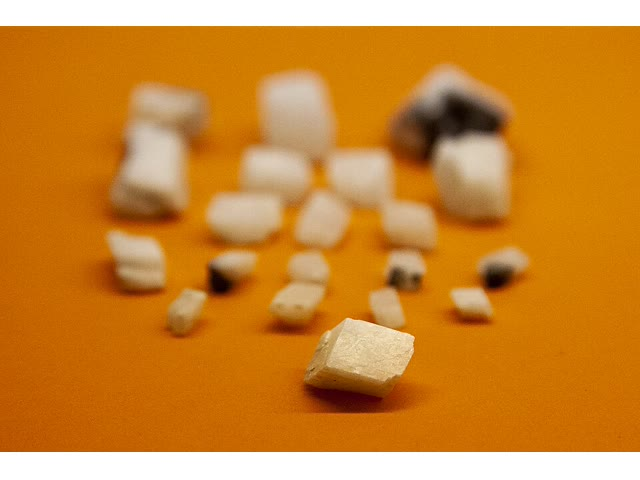
\includegraphics[width=\linewidth]{images/book3/b1-mineral-calcite-rhombs.jpg}

{\scriptsize Romboedros de exfoliación de calcita. Fotografía de Giovanna Canu y Eva Santini, CC BY 4.0
(Wikimedia Commons).}
\end{minipage}
\end{inthelab}

\begin{omfigure}
\setlength{\tabcolsep}{2pt}
\begin{tabular}{ccc}
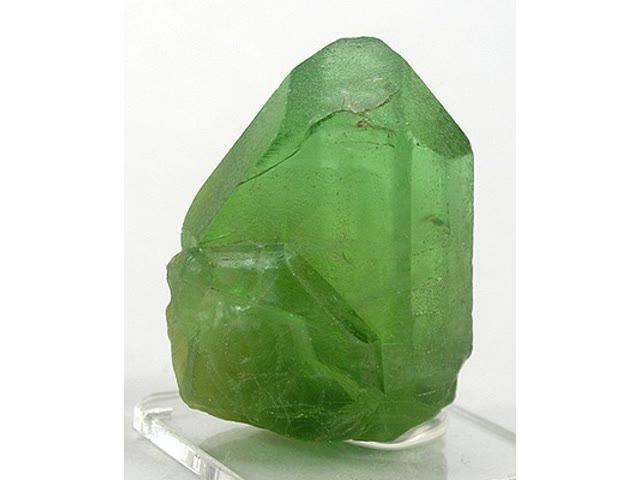
\includegraphics[width=0.31\linewidth]{images/book3/b1-mineral-olivine.jpg} &
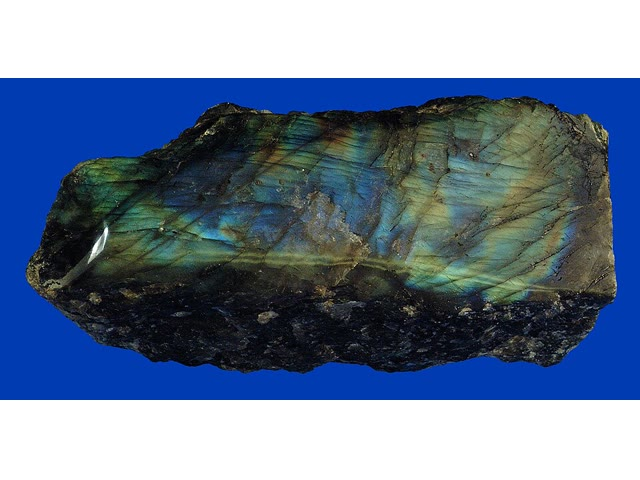
\includegraphics[width=0.31\linewidth]{images/book3/b1-mineral-plagioclase.jpg} &
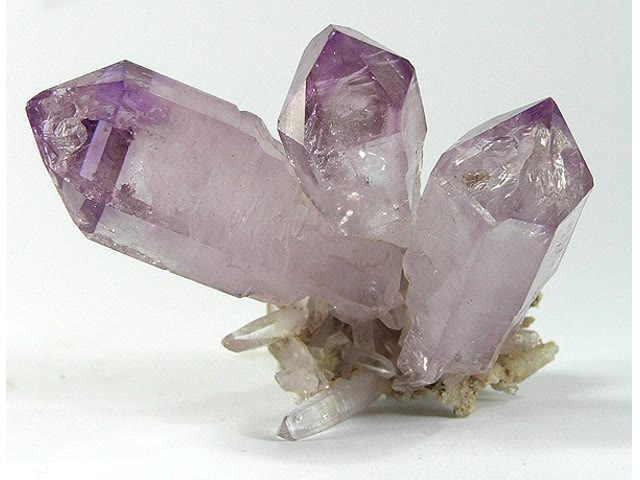
\includegraphics[width=0.31\linewidth]{images/book3/b1-mineral-quartz.jpg} \\
{\small (a) \omterm{def:b1:rock-forming-minerals:groups}{olivino}} & {\small (b) \omterm{def:b1:rock-forming-minerals:groups}{plagioclasa} (labradorita)} & {\small (c) cuarzo (amatista)} \\[4pt]
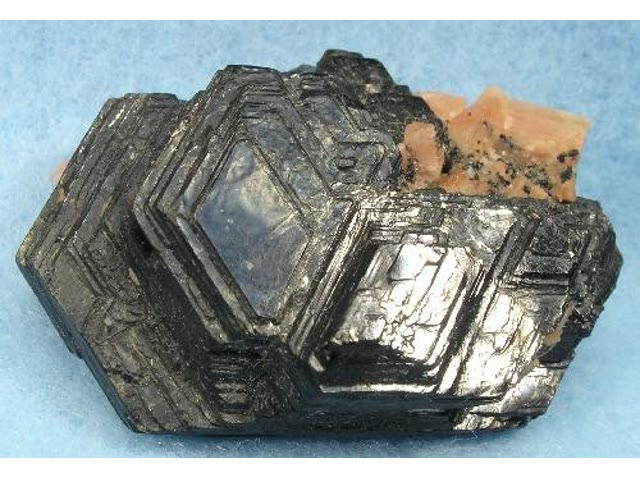
\includegraphics[width=0.31\linewidth]{images/book3/b1-mineral-biotite.jpg} &
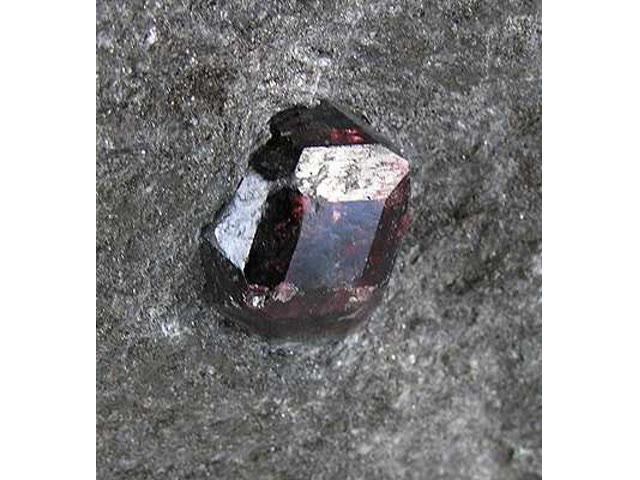
\includegraphics[width=0.31\linewidth]{images/book3/b1-mineral-garnet.jpg} &
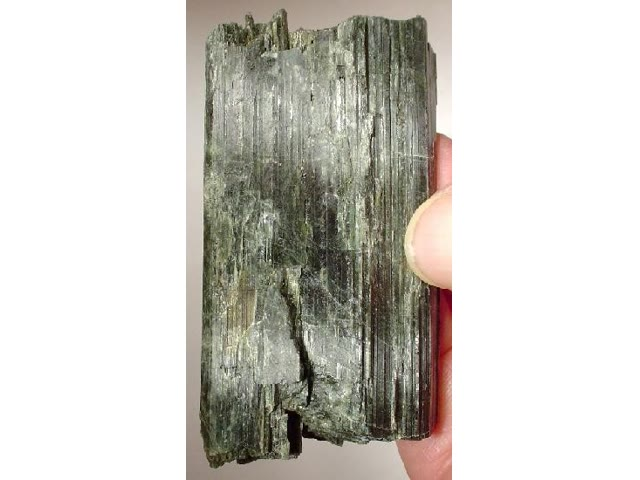
\includegraphics[width=0.31\linewidth]{images/book3/b1-mineral-hornblende.jpg} \\
{\small (d) biotita sobre ortoclasa} & {\small (e) \omterm{def:b1:rock-forming-minerals:groups}{granate} (almandino)} & {\small (f) hornblenda} \\
\end{tabular}
\medskip
% ledger: commons:min-olivine, commons:min-plagioclase, commons:min-quartz, commons:min-biotite, commons:min-garnet, commons:min-hornblende

{\small Seis \omterm{def:b1:rock-forming-minerals:mineral}{minerales} formadores de rocas: (a) un cristal de \omterm{def:b1:rock-forming-minerals:groups}{olivino} de calidad gema; (b) una lámina pulida de
\omterm{def:b1:rock-forming-minerals:groups}{plagioclasa} que muestra el juego de colores de la labradorita; (c) cristales de cuarzo, prismas de seis caras con
puntas piramidales; (d) un libro de láminas de biotita sobre un cristal de ortoclasa; (e) un cristal de \omterm{def:b1:rock-forming-minerals:groups}{granate}
almandino en su matriz; (f) un prisma de hornblenda. Fotografías (a), (c)--(f) Robert M.~Lavinsky, CC BY-SA 3.0;
(b) Twyla Baker, CC0 (Wikimedia Commons).}
\end{omfigure}

\section{Ejercicios}

\begin{exercise}[$\star$]\label{exo:b1:rock-forming-minerals:1}
Nómbrese la clase de silicato de cada anión, y dése el número $s$ de vértices compartidos por cada tetraedro:
\ce{SiO4^{4-}}, \ce{Si2O7^{6-}}, \ce{Si6O18^{12-}}, \ce{Si2O5^{2-}}, \ce{SiO2}. ¿A qué clase podría pertenecer
\ce{SiO3^{2-}}?
\end{exercise}

\begin{exercise}[$\star$]\label{exo:b1:rock-forming-minerals:2}
Con los pesos atómicos O \num{15.999}, Si \num{28.085}, Mg \num{24.305} y Fe \qty{55.845}{g.mol^{-1}}, calcúlense
las masas molares de la forsterita y la fayalita, y después sus volúmenes molares a partir de las densidades
\num{3.275} y \qty{4.392}{g.cm^{-3}}.
% ledger: ciaaw:O, ciaaw:Si, ciaaw:Mg, ciaaw:Fe, hom:forsterite, hom:fayalite
\end{exercise}

\begin{exercise}[$\star$]\label{exo:b1:rock-forming-minerals:3}
En coordinación seis los radios son \ce{Mg^{2+}} \qty{0.72}{\angstrom}, \ce{Fe^{2+}} \qty{0.78}{\angstrom},
\ce{Ni^{2+}} \qty{0.69}{\angstrom}, \ce{Mn^{2+}} \qty{0.83}{\angstrom} y \ce{Ca^{2+}} \qty{1.00}{\angstrom}.
Calcúlese la diferencia de cada uno respecto del radio de \ce{Mg^{2+}} en tanto por ciento, y dígase, según las
reglas de Goldschmidt, cuáles pueden reemplazar libremente al magnesio en el \omterm{def:b1:rock-forming-minerals:groups}{olivino}.
% ledger: shannon:radii, goldschmidt:size
\end{exercise}

\begin{exercise}[$\star$]\label{exo:b1:rock-forming-minerals:4}
El grafito y el diamante tienen densidades \num{2.16} y \qty{3.51}{g.cm^{-3}}; la calcita y la aragonita,
\num{2.71} y \qty{2.93}{g.cm^{-3}}. ¿En qué porcentaje aumenta la densidad en cada cambio? ¿Qué \omterm{def:b1:rock-forming-minerals:polymorph}{polimorfo} de cada
pareja se forma a mayor presión?
% ledger: webmineral:polymorphs, hom:calcite
\end{exercise}

\begin{exercise}[$\star\star$]\label{exo:b1:rock-forming-minerals:5}
Escríbase la \omterm{def:b1:rock-forming-minerals:formula}{fórmula estructural} de la \omterm{def:b1:rock-forming-minerals:groups}{plagioclasa} $\text{An}_{30}$ (\qty{30}{\percent} de las posiciones grandes
ocupadas por calcio), y compruébese que es neutra.
\end{exercise}

\begin{exercise}[$\star\star$]\label{exo:b1:rock-forming-minerals:6}
En una cadena doble, la mitad de los tetraedros comparten dos vértices y la mitad tres. Cuéntense directamente en
el panel (f) de la figura de enlaces los oxígenos de un grupo que se repite de cuatro tetraedros, y compruébese la
fórmula \ce{Si4O11^{6-}} que da \cref{prop:b1:rock-forming-minerals:si-o}.
\end{exercise}

\begin{exercise}[$\star\star$]\label{exo:b1:rock-forming-minerals:7}
Recalcúlese en cuatro oxígenos el análisis de un \omterm{def:b1:rock-forming-minerals:groups}{olivino} \qty{40.20}{\percent} de \ce{SiO2},
\qty{47.10}{\percent} de \ce{MgO}, \qty{12.20}{\percent} de \ce{FeO} y \qty{0.40}{\percent} de \ce{NiO}
(masa molar del \ce{NiO}: \qty{74.692}{g.mol^{-1}}). Dése su \omterm{def:b1:rock-forming-minerals:formula}{fórmula estructural}, compruébese, y dése su
contenido en forsterita. Después muéstrese que el contenido en forsterita puede hallarse solo con los
porcentajes de \ce{MgO} y \ce{FeO}.
\end{exercise}

\begin{exercise}[$\star\star$]\label{exo:b1:rock-forming-minerals:8}
Compruébese que la moscovita \ce{KAl2(Si3Al)O10(OH)2} es neutra. Sus láminas de tetraedros tienen un
aluminio por cada tres silicios: ¿qué carga da esto a la lámina por unidad de fórmula, y qué ion la equilibra?
\end{exercise}

\begin{exercise}[$\star\star$]\label{exo:b1:rock-forming-minerals:9}
Con los volúmenes molares \num{42.96} y \qty{46.40}{cm^3.mol^{-1}} y las masas molares \num{140.691} y
\qty{203.771}{g.mol^{-1}}: (a) calcúlese la densidad de $\text{Fo}_{50}$ por mezcla ideal, y compárese con la
media de las densidades de los \omterm{def:b1:rock-forming-minerals:solid-solution}{términos extremos}; (b) hállese el contenido en forsterita de un \omterm{def:b1:rock-forming-minerals:groups}{olivino} de
densidad \qty{3.600}{g.cm^{-3}}.
\end{exercise}

\begin{exercise}[$\star\star\star$]\label{exo:b1:rock-forming-minerals:10}
Con la notación de \cref{prop:b1:rock-forming-minerals:ideal-mixing}, demuéstrese que
\[
  \rho(x) - \bigl(x\rho_1 + (1 - x)\rho_2\bigr) =
  \frac{x(1 - x)(\rho_1 - \rho_2)(V_1 - V_2)}{V(x)} .
\]
Dedúzcase que la densidad del \omterm{def:b1:rock-forming-minerals:groups}{olivino} queda por encima de la recta que une los \omterm{def:b1:rock-forming-minerals:solid-solution}{términos extremos}, y calcúlese
la diferencia en $\text{Fo}_{50}$.
\end{exercise}

\begin{exercise}[$\star\star\star$]\label{exo:b1:rock-forming-minerals:11}
Un \omterm{def:b1:rock-forming-minerals:groups}{plagioclasa} de un gabro da \qty{54.10}{\percent} de \ce{SiO2}, \qty{28.90}{\percent} de \ce{Al2O3},
\qty{11.20}{\percent} de \ce{CaO}, \qty{5.10}{\percent} de \ce{Na2O} y \qty{0.30}{\percent} de \ce{K2O} (masas
molares \num{60.083}, \num{101.961}, \num{56.077}, \num{61.979}, \qty{94.195}{g.mol^{-1}}). Recalcúlese en
ocho oxígenos; compruébese que los sitios tetraédricos (Si + Al) contienen 4 átomos y la posición grande
(Ca + Na + K) 1; compruébese la \omterm{def:b1:rock-forming-minerals:substitution}{sustitución acoplada} comparando $\mathrm{Al} - 1$ con Ca; dése el contenido en
anortita $100\,\mathrm{Ca}/(\mathrm{Ca} +
\mathrm{Na} + \mathrm{K})$.
\end{exercise}

\begin{exercise}[$\star\star\star$]\label{exo:b1:rock-forming-minerals:12}
Una microsonda no distingue \ce{Fe^{2+}} de \ce{Fe^{3+}} y da todo el hierro como \ce{FeO}. (a) Muéstrese que la
magnetita pura \ce{Fe3O4}, analizada así, suma un \qty{93.09}{\percent}. (b) Recalcúlese este análisis en cuatro
oxígenos, y dígase por qué el resultado es imposible para un \omterm{def:b1:rock-forming-minerals:mineral}{mineral} con tres cationes por cuatro oxígenos. (c)
Recalcúlese en tres cationes, y hállense los números de \ce{Fe^{2+}} y \ce{Fe^{3+}} exigiendo que la fórmula sea
neutra. (d) Exprésese de nuevo el análisis como \ce{FeO} y \ce{Fe2O3}, y dese el nuevo total.
\end{exercise}

\section{Problema: un olivino de un basalto}

\begin{problem}[{Problema de fin de semana --- recalcular un análisis de microsonda de un olivino, escribir y
comprobar su fórmula, y hallar su composición, su densidad y su masa en un metro cúbico de basalto}]
\label{pb:b1:rock-forming-minerals:1}
% invented analysis: figdata/bachelor-1/solid_solution.py (OLIVINE_WT); values: calc/ch07.py
% ledger: ciaaw:O, ciaaw:Si, ciaaw:Mg, ciaaw:Fe, ciaaw:Mn, ciaaw:Ni, ciaaw:Ca, hom:forsterite, hom:fayalite, shannon:radii
Los cristales verdes de un basalto son \omterm{def:b1:rock-forming-minerals:groups}{olivino}. Un análisis con microsonda de uno de ellos da, en porcentaje
en peso de óxidos:
\begin{center}
\small
\begin{tabular}{lcccccc}
\hline
óxido & \ce{SiO2} & \ce{FeO} & \ce{MnO} & \ce{MgO} & \ce{NiO} & \ce{CaO} \\
\% en masa & 39.50 & 16.53 & 0.23 & 43.32 & 0.20 & 0.22 \\
\hline
\end{tabular}
\end{center}
Los pesos atómicos son O \num{15.999}, Si \num{28.085}, Fe \num{55.845}, Mn \num{54.938}, Mg \num{24.305},
Ni \num{58.693}, Ca \qty{40.078}{g.mol^{-1}}. La forsterita tiene densidad \qty{3.275}{g.cm^{-3}} y la fayalita
\qty{4.392}{g.cm^{-3}}.

\medskip
\noindent\textbf{Parte I --- De los óxidos a los cationes.}
\begin{enumerate}
  \item Calcúlense las masas molares de los seis óxidos.
  \item Calcúlese el total del análisis. ¿Qué habría sugerido un total de \qty{97}{\percent}?
  \item Calcúlense los moles de cada óxido en \qty{100}{g} de \omterm{def:b1:rock-forming-minerals:groups}{olivino}.
  \item Calcúlense los moles de oxígeno que contienen, y su suma.
  \item Calcúlense los moles de cada catión.
  \item Calcúlese el factor que lleva los oxígenos a cuatro.
  \item Dése el número de átomos de cada elemento por cuatro oxígenos, con tres decimales.
\end{enumerate}

\medskip
\noindent\textbf{Parte II --- La fórmula estructural.}
\begin{enumerate}[resume]
  \item El \omterm{def:b1:rock-forming-minerals:groups}{olivino} tiene una posición tetraédrica y dos octaédricas por cuatro oxígenos. Calcúlese la suma de los
        cationes distintos del silicio, y compárense ambos totales de posiciones con la fórmula ideal.
  \item Escríbase la \omterm{def:b1:rock-forming-minerals:formula}{fórmula estructural} del \omterm{def:b1:rock-forming-minerals:groups}{olivino}.
  \item Compruébese que la fórmula es neutra, y explíquese por qué esta comprobación, a diferencia de la de la
        pregunta 8, no podría haber fallado.
  \item Con los radios iónicos (\ce{Mg^{2+}} \qty{0.72}{\angstrom}, \ce{Fe^{2+}} \qty{0.78}{\angstrom},
        \ce{Ni^{2+}} \qty{0.69}{\angstrom}, \ce{Mn^{2+}} \qty{0.83}{\angstrom}, \ce{Ca^{2+}} \qty{1.00}{\angstrom},
        todos en seis coordinaciones), explíquese por qué el níquel es frecuente en el \omterm{def:b1:rock-forming-minerals:groups}{olivino} y el calcio raro.
  \item La microsonda da todo el hierro como \ce{FeO}. Explíquese por qué el número total de cationes hallado en la
        pregunta 7 muestra que el \omterm{def:b1:rock-forming-minerals:groups}{olivino} no contiene \ce{Fe^{3+}} significativo.
\end{enumerate}

\medskip
\noindent\textbf{Parte III --- La composición.}
\begin{enumerate}[resume]
  \item Calcúlese el contenido en forsterita $\mathrm{Fo} = 100\,\mathrm{Mg}/(\mathrm{Mg} +
        \mathrm{Fe})$, con un decimal.
  \item ¿Cuál es el \omterm{def:b1:rock-forming-minerals:formula}{número de Mg} del \omterm{def:b1:rock-forming-minerals:groups}{olivino}? ¿Por qué es igual aquí al contenido en forsterita?
  \item Escríbase el \omterm{def:b1:rock-forming-minerals:groups}{olivino} como una \omterm{def:b1:rock-forming-minerals:solid-solution}{solución sólida} binaria $\mathrm{Fo}_x\mathrm{Fa}_{1-x}$, ignorando Mn, Ni y
        Ca, y dése la proporción de sus posiciones octaédricas ocupadas por hierro.
  \item Muéstrese que el contenido en forsterita puede calcularse solo con los porcentajes de \ce{MgO} y \ce{FeO},
        sin el factor de la pregunta 6, y hágase.
  \item Un \omterm{def:b1:rock-forming-minerals:groups}{olivino} que creció más tarde en la misma lava tiene \qty{40.5}{\percent} de \ce{MgO} y
        \qty{20.0}{\percent} de \ce{FeO}. Calcúlese su contenido en forsterita. ¿Qué \omterm{def:b1:rock-forming-minerals:groups}{olivino} es más rico en hierro?
\end{enumerate}

\medskip
\noindent\textbf{Parte IV --- Densidad y masa.}
\begin{enumerate}[resume]
  \item Calcúlense las masas molares y los volúmenes molares de la forsterita y la fayalita (volúmenes molares con
        dos decimales).
  \item Tomando el \omterm{def:b1:rock-forming-minerals:groups}{olivino} como el binario $\mathrm{Fo}_x\mathrm{Fa}_{1-x}$ de la pregunta 15, con $x$ redondeado a
        tres decimales, calcúlense su masa molar y su volumen molar por mezcla ideal.
  \item Dedúzcase su densidad, con tres decimales.
  \item Compárese con la interpolación lineal entre las densidades de los \omterm{def:b1:rock-forming-minerals:solid-solution}{términos extremos}.
  \item El basalto contiene un \qty{12}{\percent} de \omterm{def:b1:rock-forming-minerals:groups}{olivino} en volumen. ¿Qué masa de \omterm{def:b1:rock-forming-minerals:groups}{olivino} contiene un metro
        cúbico del basalto?
  \item El basalto tiene una densidad de \qty{2.95}{g.cm^{-3}}. ¿Cuál es la proporción de \omterm{def:b1:rock-forming-minerals:groups}{olivino} en masa?
  \item ¿Cuál es el contenido en forsterita del \omterm{def:b1:rock-forming-minerals:groups}{olivino}, redondeado al entero por ciento?
\end{enumerate}
\end{problem}
